\documentclass[11pt]{article}
\usepackage[margin=1in]{geometry}
\usepackage{graphicx}
\usepackage{amsmath,amssymb,amsthm,mathtools}
\IfFileExists{lmodern.sty}{\usepackage{lmodern}}{}
\usepackage[expansion=false]{microtype}
\usepackage{booktabs,array}
\usepackage{enumitem}
\usepackage{xcolor}
\usepackage[colorlinks=true,linkcolor=blue!50!black,citecolor=green!35!black,urlcolor=blue!50!black]{hyperref}
\usepackage[nameinlink]{cleveref}

\newtheorem{theorem}{Theorem}[section]
\newtheorem{proposition}[theorem]{Proposition}
\newtheorem{lemma}[theorem]{Lemma}
\newtheorem{corollary}[theorem]{Corollary}
\theoremstyle{definition}
\newtheorem{definition}[theorem]{Definition}
\newtheorem{example}[theorem]{Example}
\theoremstyle{remark}
\newtheorem{remark}[theorem]{Remark}
\newtheorem*{mainthm}{Main results}

\newcommand{\D}{\mathsf{D}}
\newcommand{\R}{\mathbb{R}}
\newcommand{\Z}{\mathbb{Z}}
\newcommand{\Cpl}{\operatorname{Cpl}}
\newcommand{\diag}{\operatorname{diag}}
\newcommand{\T}{\mathsf T}
\newcommand{\Hess}{\operatorname{Hess}}

\title{Bridges:\\ From Probability and Entropy to Branes, with Worked Examples}
\author{Vinay K. Awasthi\\
Department of Applied Mathematics and Statistics\\
Johns Hopkins University\thanks{Code and checks: \url{https://github.com/vkawasth/Trainingless-Transformer-NoGradientDescent/tree/main/bridges}. \texttt{check\_bridges.py} (16 checks) verifies numerically the computable statements proved here, on examples
and random instances, and every number in the worked examples. Propositions 5.2, 5.3 and 5.5, beyond the elementary criterion checked in H2, and the derived invariants in
Proposition 7.1 rest on the cited literature, as do the imported theorems (T1)--(T8) of Section 8; results cited from the other papers are checked there.}}
\date{October 8, 2026, draft 4}

\begin{document}
\maketitle

\begin{abstract}
We construct the maps between five layers, probability, information geometry, entropy, couplings and symplectic branes,
and test which structures they preserve. Entropy's negative Hessian is the Fisher metric. Marginal constraints become
Lagrangian branes as conormal bundles, and the graph of the entropy differential meets such a brane exactly at the
maximum-entropy law of the constraint, transversally because the Fisher metric is nondegenerate. When no positive law meets
the constraint the brane is empty. In a worked example with three bits this happens exactly when the pairwise disagreement
reaches $2/3$, the contextual fraction is $1-3\varepsilon$ below the threshold, and the Fisher form of the fibre blows up as
the threshold is approached. Because a cell of the filler vanishes there, joint samples detect the boundary at distance $m$
from $O(1/m)$ samples, while pairwise-only samples need $O(1/m^2)$. When the same variable may be measured differently in
different contexts, Contextuality-by-Default noncontextuality is again a constraint brane, on a face of the simplex: for three bits, direct
influences of size $\Delta$ move the threshold to $\frac13-\frac{\Delta}6$, a test that ignores them reads them as contextuality, and a
decision under uncertainty needs a model of the direct influences. On the toric side,
entropy is an admissible symplectic potential on the toric manifold of every nondegenerate coupling polytope, without the
facet hypothesis of earlier work, so couplings are the points of a positive real Lagrangian and the bases of torus branes; for $2\times2$ couplings the real and torus
branes pair nontrivially only over the Fréchet midpoint, with both the positive and the negative intersection point surviving. When the
toric manifold is Fano, only the torus branes at critical points of the disc potential are nonzero objects; for $2\times2$
couplings this is the Fréchet midpoint, which is generally not the product coupling. Gluing with a fixed coupling acts on couplings linearly, and it preserves the lattice of the
torus exactly when its kernel is deterministic or constant. So gluing with a non-constant stochastic kernel is not induced by a
torus-equivariant correspondence, a defect related to, though not identical with, the defects of stochastic kernels found in
other layers of the programme. Finally we organize the Floer theory of couplings in layers whose hypotheses are checked case by case.
Every $2\times3$ coupling polytope gives a Fano surface, and for rational margins its disc potential is Morse with one critical point per vertex;
for generic margins the nonzero torus branes lie over couplings where three cells, or the two cells of a column, are smallest and equal; they
never lie over the product coupling when its smallest facet cell is unique; and in all computed cases over the leximin coupling, the coupling lexicographically farthest from breaking, which
usually carries most of them. For every $3\times3$ margin the toric $4$-fold is semi-Fano, and by the Chan--Lau--Leung--Tseng formula its disc
potential has no corrections, so the same computation applies. We give the topology and Maslov indices of the real locus, which for
$2\times3$ and $3\times3$ couplings is non-orientable except in the $\mathbb{CP}^1\times\mathbb{CP}^1$ chambers, and reduce the sheaf model of the
entropy brane to the admissibility of one explicit isotopy. Finally we compute these objects for margins from public data (NHANES and the
General Social Survey): their toric surfaces, nonzero torus branes, entropy brane and its steepness.
\end{abstract}

\tableofcontents

%=====================================================================
\section{Introduction}\label{sec:intro}
%=====================================================================

The programme of which this note is part works with five layers:
\begin{itemize}[leftmargin=*,nosep]
\item probability distributions, which describe states and uncertainty;
\item information geometry, which measures how distinguishable nearby states are;
\item entropy, which supplies a potential and selects canonical distributions;
\item coupling spaces, which describe compatible joint realizations \cite{Conditionals,Algebras};
\item symplectic branes and their Fukaya-type categories, which could organize admissible structures, transformations and
  their higher compositions \cite[\S\S7, 10]{Conditionals}.
\end{itemize}
The task is to construct the maps between the layers and to find out which structures they preserve. Each bridge below
comes with a proof and a worked example in which every number can be checked by hand; the one bridge where data enter, the
detection of a breaking point, comes with a synthetic test.

\begin{mainthm}
\leavevmode
\begin{enumerate}[label=(\Alph*),leftmargin=*]
\item \emph{Constraint branes} (\cref{thm:conormal}). The conormal bundle of a marginal constraint is a Lagrangian in the
  cotangent bundle of the open simplex. The graph of $dH$ meets it in exactly one point, the maximum-entropy law of the
  constraint, transversally; it misses it exactly when no positive law satisfies the constraint.
\item \emph{Three bits} (\cref{ex:threebits}). For pairwise disagreement $1-\varepsilon$, a joint exists iff $\varepsilon\ge\frac13$, a
  positive one iff $\frac13<\varepsilon<1$; the contextual fraction is $1-3\varepsilon$ below $\frac13$; the Fisher form of the fibre is
  $\frac8{3\varepsilon-1}+\frac{24}{1-\varepsilon}$; and from joint samples the threshold is detected at distance $m$ with $O(1/m)$ samples.
\item \emph{Contextuality by Default} (\cref{prop:cbdbrane,ex:cbd3}). CbD-noncontextuality is a constraint brane on a face of the simplex.
  For three bits, direct influences of size $\Delta$ move the threshold to $\frac13-\frac{\Delta}6$; a naive test that ignores them misreads them as
  contextuality, and with uncertain direct influences the decision needs a model for them.
\item \emph{Toric branes} (\cref{thm:abreu,prop:realpositive,prop:floer}). On the toric manifold of every nondegenerate
  coupling polytope, entropy is an admissible symplectic potential; couplings are the points of the positive real Lagrangian
  and the bases of the torus branes; when the manifold is Fano, only torus branes at critical points of the disc potential
  survive, which for $2\times2$ couplings is the Fréchet midpoint (\cref{ex:twobytwo}).
\item \emph{Correspondences} (\cref{thm:integral,ex:gluetwo}). Gluing with a coupling whose kernel is $K$ maps lattice to
  lattice iff $K$ is deterministic or constant, so a non-constant stochastic $K$ is not induced by an equivariant correspondence; in the $2\times2$ case it scales the moment segment by the Dobrushin coefficient.
\item \emph{Categorical layer} (\cref{prop:morita}). The gluing algebra is Morita equivalent to $\R\times\R$, so all its derived
  invariants are those of two points.
\item \emph{A modular Floer theory} (\cref{sec:modular}). With hypotheses checked for couplings: all $2\times3$ toric surfaces are Fano
  (\cref{prop:fano23}), with Morse potentials for rational margins and two kinds of brane position for generic ones, and the product coupling
  carries no brane when its smallest facet cell is unique; in the computed cases the leximin coupling always carries one (\cref{thm:sweep23}). All $3\times3$ toric $4$-folds are
  semi-Fano with no disc-potential corrections (\cref{thm:nocorr}). The real locus is non-orientable except for $\mathbb{CP}^1\times\mathbb{CP}^1$
  (\cref{prop:reallocus}). The entropy brane is exactly isotopic to a standard brane, with one transverse intersection throughout; whether the
  isotopy is admissible is open (\cref{prop:sheaf}).
\end{enumerate}
\end{mainthm}

\paragraph{What is not claimed.} We do not construct a functor from couplings to a Fukaya category. We show where the obvious
candidates fail and why: in the cotangent bundle of the simplex, which is contractible, the entropy brane carries only its one
intersection point; in the Fano case, torus branes over most couplings are zero objects; and gluing with a non-constant
stochastic kernel is not induced by an equivariant correspondence of the kind defined in \cref{sec:correspondences}.
Non-equivariant correspondences are not ruled out.

%=====================================================================
\section{From probability to geometry}\label{sec:geometry}
%=====================================================================

Let $\Delta^\circ$ be the open simplex of full-support distributions on $n$ points, with tangent space
$T=\{u:\sum u_y=0\}$, and $H(p)=-\sum p_y\log p_y$.

\begin{proposition}\label{prop:fisher}
For $u,v\in T$, $-d^2H_p(u,v)=\sum_yu_yv_y/p_y$, the Fisher metric.
\end{proposition}
\begin{proof}
$\partial^2H/\partial p_y\partial p_z=-\delta_{yz}/p_y$.
\end{proof}

The Fisher metric is symmetric, so it is not a symplectic form; the two structures coexist in the cotangent bundle, the
metric on the base and the canonical form $\omega=\sum dp_y\wedge d\xi_y$ on $T^*\Delta^\circ$, and on the toric manifolds of
\cref{sec:toric}, where the Fisher metric is twice the Kähler metric on the real section \cite[Prop.~6.5]{Conditionals}.

%=====================================================================
\section{Constraint branes in the cotangent bundle}\label{sec:conormal}
%=====================================================================

A marginal constraint fixes a linear image $Mp=b$ of the law. Its \emph{fibre} is $C=\{p\in\Delta:Mp=b\}$ and its open part is
$C^\circ=C\cap\Delta^\circ$. The fibre is not Lagrangian, but its conormal bundle is, as for every submanifold
\cite{McDuffSalamon2017}:
\[
N^*C^\circ=\{(p,\xi)\in T^*\Delta^\circ:p\in C^\circ,\ \xi\vert_{T_pC}=0\},\qquad T_pC=\ker M\cap T.
\]
The \emph{entropy brane} is the graph $L_H=\{(p,dH_p)\}$, an exact Lagrangian.

\begin{theorem}[Conormal intersection]\label{thm:conormal}
If $C^\circ\neq\emptyset$, then $L_H\cap N^*C^\circ$ is the single point over the maximum-entropy law $p^\star$ of $C$, and the
intersection is transversal. If $C^\circ=\emptyset$, then $N^*C^\circ=\emptyset$ and the intersection is empty, although $C$ itself may
be nonempty.
\end{theorem}
\begin{proof}
A point $(p,dH_p)$ lies in $N^*C^\circ$ iff $dH_p$ vanishes on $T_pC$, that is, iff $p$ is a critical point of $H$ on the
relatively open convex set $C^\circ$. $H$ is strictly concave, so there is at most one such point, and it is the maximizer of $H$
over $C$; the maximizer lies in $C^\circ$ when $C^\circ\ne\emptyset$, because the derivative of $H$ in a direction that raises a
vanishing coordinate is $+\infty$. Transversality of the graph of $dH$ to a conormal bundle at a point is nondegeneracy of the
Hessian of $H\vert_C$ there, and by \cref{prop:fisher} that Hessian is minus the Fisher metric on $T_pC$, which is definite.
\end{proof}

\begin{corollary}\label{cor:filler}
Suppose the margins admit a strictly positive joint law, so that $C^\circ\ne\emptyset$. For the chain margins $(X,Y)$ and $(Y,Z)$ the intersection point is the conditionally independent gluing
$P_{XY}P_{YZ}/P_Y$, the canonical filler of \cite[Thm.~4.2]{Conditionals}. For pairwise margins of three variables it is the
limit of iterative proportional fitting started at the uniform law \cite{Csiszar1975}.
\end{corollary}
\begin{proof}
The gluing has the margins, and $\log$ of it is a sum of a function of $(x,y)$ and one of $(y,z)$, which is orthogonal to the
kernel of the marginal map. The second statement is the maximum-entropy characterization of fitting.
\end{proof}

So the brane picture of compatibility is exact: a constraint is compatible with positive laws iff its brane is nonempty, and
then it meets the entropy brane exactly once, at the canonical filler.

\paragraph{Support floors move the intersection out of reach.} A support policy asks for a filler with every cell at least $\tau$. The intersection point above, the canonical filler, can fail
the floor while other fillers meet it: for binary chains a floored filler exists iff $\tau\le\tfrac12\min(\min P_{XY},\min P_{YZ})$, while
the canonical filler meets the floor iff $\tau\le\min P_{XY}P_{YZ}/P_Y$ \cite[Prop.~4.7]{Conditionals}. Between the two thresholds the
entropy brane meets the constraint brane outside the admissible region, and the most uncertain admissible law is no longer the
canonical filler. On cyclic covers the floor can also exclude every global section of a family that glues
\cite[Thm.~4.8]{Conditionals}; this was observed for $24\%$ of random gluable triangles \cite[Section~14]{Validation}.


\begin{example}[Three bits]\label{ex:threebits}
Let $X_0,X_1,X_2$ be bits, each uniform, and let each pair disagree with probability $1-\varepsilon$, so that each pairwise table is
$\bigl(\begin{smallmatrix}\varepsilon/2&(1-\varepsilon)/2\\(1-\varepsilon)/2&\varepsilon/2\end{smallmatrix}\bigr)$.
\begin{enumerate}[label=(\roman*)]
\item \emph{The fibre.} The kernel of the marginal map on $\R^8$ is spanned by the parity vector $x(s)=(-1)^{\lvert s\rvert}$, so the fibre
  is a segment along $x$.
\item \emph{Threshold.} Every assignment of three bits makes $0$ or $2$ of the three pairs disagree, so the expected number of
  disagreeing pairs, $3(1-\varepsilon)$, is at most $2$: a joint exists iff $\varepsilon\ge\frac13$. At $\varepsilon=\frac13$ the only joint puts no
  mass on $000$ and $111$, and at $\varepsilon=1$ the only joint lives on $000$ and $111$; in both cases $C^\circ=\emptyset$ and the brane is
  empty. A positive joint exists iff $\frac13<\varepsilon<1$. The two ends are the breaking regime of \cite{Bands}.
\item \emph{The filler.} For $\frac13<\varepsilon<1$ the maximum-entropy law gives $a=\frac{3\varepsilon-1}4$ to $000$ and $111$ and $b=\frac{1-\varepsilon}4$
  to the six other assignments, since then $\sum_sx(s)\log p(s)=0$.
\item \emph{Transversality and its loss.} The Fisher form of the fibre at the filler is
  $\sum_sx(s)^2/p(s)=\frac8{3\varepsilon-1}+\frac{24}{1-\varepsilon}$, which is $64$ at $\varepsilon=\frac12$, $197$ at $0.35$ and $436$ at $0.34$, and
  diverges at both ends: the intersection becomes infinitely steep before it disappears.
\item \emph{Contextual fraction.} Below the threshold the contextual fraction of \cite{AbramskyBarbosaMansfield2017} is $1-3\varepsilon$.
  A sub-normalized common joint $\lambda q$ below the tables puts at most $\varepsilon$ on the agreements of each pair, and every
  assignment agrees on some pair, so $\lambda\le3\varepsilon$; the measure $3\varepsilon$ times the uniform law on the six assignments that agree on
  exactly one pair attains it.
\end{enumerate}
\end{example}

\paragraph{Synthetic test: detecting the boundary.} Take the positive law with $\varepsilon=\frac13+m$ and $N$ joint samples of the three bits,
and estimate $\varepsilon$ by the mean agreement rate. Each sample agrees on one pair, or on three if it is $000$ or $111$, so $\hat\varepsilon\le\frac13$
exactly when no all-equal sample appears, which happens with probability $(1-\frac32m)^N\approx e^{-3Nm/2}$. For $m=0.02$ and $N=25,100,400$ the
verdict ``no positive filler'' was returned in $47\%$, $6\%$ and $0\%$ of $2000$ replicates, against $46.7\%$, $4.8\%$ and $0\%$ predicted. So
$O(1/m)$ joint samples suffice. The reason is that the filler's cells on $000$ and $111$ vanish at the boundary: the Fisher information of
$\varepsilon$ in the joint model, $\frac9{2(3\varepsilon-1)}+\frac3{2(1-\varepsilon)}$, diverges there, and the test reduces to seeing a rare cell.

The rate depends on the design. In the usual contextuality design each pair is observed in its own samples, the agreement count of each
pair is binomial, its Fisher information stays bounded at the boundary, and the misses decay only once $Nm^2$ is large: $42\%$, $26\%$, $7\%$
and $0.05\%$ for $N=25,100,400,1600$. Interior walls behave in the same way; for them \cite[Prop.~12.2]{Conditionals} shows that $N$ of order
$1/m^2$ suffices.

%=====================================================================
\section{Contextuality by Default}\label{sec:cbd}
%=====================================================================

The contextual fraction of \cref{ex:threebits} assumes that a quantity measured in two contexts has the same distribution in both:
the system is \emph{consistently connected}. Real data, and decisions made from them, rarely grant this. A question asked after another
one, a lab ordered for sicker patients, a forecast scored on revised data: the context changes the distribution of what is measured.
Contextuality-by-Default (CbD) \cite{DzhafarovKujala2016} treats this case. Each measurement is a random variable labelled by its content,
what is measured, and its context, the conditions of measurement. The variables sharing a content form a \emph{connection}. Differences between
the distributions within a connection are \emph{direct influences} of the context on the measurement; contextuality is what remains after
direct influences are allowed for as fully as possible.

\begin{definition}\label{def:cbd}
A system is \emph{CbD-noncontextual} if there is a joint law of all its variables whose restriction to each context is the observed law
and in which the two variables of each connection are \emph{maximally coupled}: they differ with probability equal to the total variation
distance between their laws, the least possible.
\end{definition}

\begin{proposition}[CbD as a constraint brane]\label{prop:cbdbrane}
\begin{enumerate}[label=(\roman*)]
\item CbD-noncontextuality is the nonemptiness of a fibre $C_m$ of a marginal map, the one that records the context tables and the
  connection tables, with each connection table pinned to the maximal coupling of its two laws.
\item For binary variables a maximal coupling has a zero cell, two if the laws agree. So $C_m$ lies in a face of the simplex, and
  \cref{thm:conormal} applies inside the relative interior of that face: when the face carries a law of full support on it, the entropy
  graph meets the conormal brane of $C_m$ exactly once, at the maximum-entropy CbD coupling.
\item For a consistently connected system the maximal couplings are the diagonal ones, identifying the two variables of each
  connection reduces $C_m$ to the traditional marginal problem, and CbD-contextuality agrees with contextuality in the sense of
  \cite{AbramskyBrandenburger2011}, as in \cite{DzhafarovKujala2016}.
\end{enumerate}
\end{proposition}
\begin{proof}
(i) is \cref{def:cbd}. (ii) If two binary laws have $P(W=1)=a\le b=P(V=1)$, their maximal coupling puts $b-a$ on $(W,V)=(0,1)$ and nothing on
$(1,0)$. Restricted to the face where these cells vanish, the constraints are again linear, and the proof of \cref{thm:conormal} applies
verbatim. (iii) If $a=b$ both off-diagonal cells vanish, so the two variables are equal almost surely in every law of $C_m$.
\end{proof}

For a \emph{cyclic system} of rank $n$, contents $q_1,\dots,q_n$ and contexts $\{q_i,q_{i+1}\}$ with binary variables $V_i,W_{i+1}$ valued in
$\pm1$, Kujala and Dzhafarov proved the criterion \cite{KujalaDzhafarov2016}: the system is contextual iff
\[
s_{\mathrm{odd}}\bigl(\langle V_1W_2\rangle,\dots,\langle V_nW_1\rangle\bigr)>(n-2)+\Delta,\qquad \Delta=\sum_i\bigl\lvert\langle V_i\rangle-\langle W_i\rangle\bigr\rvert,
\]
where $s_{\mathrm{odd}}(x)$ is the largest $\sum_i\pm x_i$ with an odd number of minus signs, and its degree of contextuality is
$\mathrm{CNTX}=\frac12\max\bigl(0,\ s_{\mathrm{odd}}-(n-2)-\Delta\bigr)$ \cite{KujalaDzhafarov2019}. The linear program of
\cref{prop:cbdbrane}(i) and the criterion agree on all $950$ random cyclic systems of rank $3$ and $4$ we tried, $364$ of them contextual.

\begin{example}[Three bits with direct influences]\label{ex:cbd3}
Modify \cref{ex:threebits} so that in context $\{q_i,q_{i+1}\}$ the first variable has $P(V_i=1)=\frac12+\frac d2$ while $W_{i+1}$ stays uniform,
with pairwise disagreement $1-\varepsilon$ as before. Then $\Delta=3d$ and $s_{\mathrm{odd}}=3(1-2\varepsilon)$ for $\varepsilon<\frac12$, so the system is
contextual iff
\[
\varepsilon<\tfrac13-\tfrac{\Delta}6 .
\]
Direct influences lower the threshold: $\frac13$, $0.283$ and $0.233$ for $d=0$, $0.1$ and $0.2$. On the consistently connected path $d=0$,
$\mathrm{CNTX}=1-3\varepsilon$, the contextual fraction of \cref{ex:threebits}. At $\varepsilon=0.30$ and $d=0.2$ the tables admit no common joint of the
traditional kind (the least $L^1$ adjustment that makes them compatible is $0.40$), yet the system is CbD-noncontextual: the
incompatibility is entirely due to direct influences.
\end{example}

This is the distinction the clinical protocol of \cite[\S11]{Bands} needs: incompatibility of observed margins splits into sampling,
direct influences of the context (selection, disturbance, framing), and a residual that only then deserves the name contextuality.

\paragraph{Contextuality under uncertainty.} A decision that depends on whether a system is contextual must be made from samples. Take
$N$ samples from each context of \cref{ex:cbd3}, put independent uniform Dirichlet priors on the three context tables, and compute the posterior
probability that the system is contextual, by the CbD criterion and by the naive criterion $s_{\mathrm{odd}}>n-2$ that ignores direct
influences:
\begin{center}
\begin{tabular}{lccc}
\toprule
true system & $N=100$ & $N=400$ & $N=1600$\\
\midrule
CbD-noncontextual, $\varepsilon=0.30$, $d=0.2$ & $0.04$ / $0.79$ & $0.00$ / $0.99$ & $0.00$ / $0.99$\\
CbD-contextual, $\varepsilon=0.25$, $d=0.1$ & $0.83$ / $1.00$ & $0.95$ / $1.00$ & $1.00$ / $1.00$\\
contextual, consistent, $\varepsilon=0.32$, $d=0$ & $0.08$ / $0.59$ & $0.06$ / $0.79$ & $0.57$ / $1.00$\\
\bottomrule
\end{tabular}
\end{center}
(Entries are CbD / naive.) The naive criterion reads direct influences as contextuality with near certainty. The CbD criterion with the
estimated $\Delta$ is conservative near the threshold: sampling noise makes the estimated $\Delta$ positive even when the true one is $0$, and
noise is then absorbed as direct influence. So a decision under uncertainty needs a model of the direct influences themselves, for example
a prior probability that the system is consistently connected, and acts on contextuality when its posterior probability exceeds
$L_{\mathrm{wrong\ global}}/(L_{\mathrm{wrong\ global}}+L_{\mathrm{needless\ split}})$, the ratio of the costs of the two errors.

Two remarks on design. Contextuality cannot be detected from a single joint source: if all variables are sampled together, the empirical
joint is a global section \cite[Thm.~1.1]{ThreeLayers}. The fast $O(1/m)$ detection with joint samples in \cref{sec:conormal} therefore
concerns positivity on the compatible side of the threshold, not contextuality; tests of contextuality use separate samples per context, at
the $O(1/m^2)$ rate.

%=====================================================================
\section{Toric branes}\label{sec:toric}
%=====================================================================

For nondegenerate margins $f,g$, the coupling polytope $\Cpl(f,g)$ is Delzant for the lattice of integer circulations, and it is
the moment polytope of a compact toric manifold $X_{f,g}$ \cite[Thm.~6.4]{Conditionals}, \cite{Delzant1988}. The fibre of the moment
map over an interior coupling is a Lagrangian torus. A symplectic potential on the polytope determines a compatible toric
Kähler structure when it satisfies Abreu's conditions \cite{Abreu2003}: it differs from Guillemin's potential
$G_P=\frac12\sum_{\text{facets}}\ell\log\ell$ \cite{Guillemin1994} by a function smooth on the closed polytope, its Hessian is
positive definite inside, and $\det(\Hess G)\prod_{\text{facets}}\ell$ is smooth and positive on the closed polytope.

\begin{theorem}[Entropy is an admissible potential]\label{thm:abreu}
For nondegenerate margins, every cell $\alpha_c$ is either a facet function of $\Cpl(f,g)$ or strictly positive on it, and
$G=\frac12\sum_c\alpha_c\log\alpha_c=-\frac12H$ satisfies Abreu's conditions. Hence it defines a compatible toric Kähler structure on
$X_{f,g}$ whose metric on the real section is half the Fisher metric, and whose potential has the product coupling as its unique
critical point.
\end{theorem}
\begin{proof}
The polytope is simple, and at each vertex exactly $(n-1)(m-1)$ cells vanish, as many as the dimension. At a vertex of a simple
polytope given by a system in which exactly $d$ inequalities are tight, each tight inequality defines a facet. Every face on which
$\alpha_c=0$ contains a vertex where it is tight, so $\alpha_c$ is a facet function or never vanishes. In the second case
$\alpha_c\log\alpha_c$ is smooth on the polytope, so $G-G_P$ is smooth. The Hessian is $\frac12\sum_c u_c^2/\alpha_c$ on circulations, which is
positive definite. Near a vertex, in Delzant coordinates in which the facets through it are $x_i\ge0$ (each cell
function is primitive on the lattice of integer circulations, since a basic move takes the value $1$ on it, and distinct cells give
distinct facets off the walls), $\Hess G=\frac12X^{-1}+S$
with $X=\diag(x)$ and $S$ smooth and positive semidefinite, so $\det(\Hess G)\prod x_i=\det(\frac12I+XS)$ is smooth and at least
$2^{-d}$. A boundary point is covered by the coordinates of a vertex of its minimal face, in which the remaining facet functions
are positive factors. The critical point is computed in \cite[Prop.~6.5]{Conditionals}.
\end{proof}

This removes the hypothesis of \cite[Prop.~6.5]{Conditionals} that every cell be a facet. Guillemin's own potential is a
different admissible potential, and when some cells are not facets its critical point may differ from the product coupling
(\cref{ex:twobytwo}).

\begin{proposition}[The real Lagrangians]\label{prop:realpositive}
The real locus $X_{f,g}^{\R}$, the fixed set of complex conjugation, is a closed Lagrangian submanifold of dimension $d=(n-1)(m-1)$. Its
positive part $X_{f,g}^{>0}$, inside the open torus orbit, is an open Lagrangian whose closure is mapped homeomorphically onto
$\Cpl(f,g)$ by the moment map \cite{Fulton1993}. The torus brane $L_u$ over an interior coupling $u$ meets $X_{f,g}^{\R}$ transversally in the
$2^d$ points whose angle coordinates lie in $\{0,\pi\}^d$, exactly one of them in the positive part. So the couplings are the points of one
open Lagrangian, and each is the positive one of the intersection points of the closed real Lagrangian with a torus brane.
\end{proposition}
\begin{proof}
Complex conjugation is antiholomorphic and preserves the torus-invariant Kähler form up to sign, so its fixed set is Lagrangian. The
homeomorphism is the classical statement about the nonnegative part of a projective toric variety. In action--angle coordinates
conjugation sends the angles $\theta$ to $-\theta$, whose fixed points on a fibre are $\theta\in\{0,\pi\}^d$; the positive part is $\theta=0$.
Transversality holds because the real locus is a section of the fibration over the interior of the polytope.
\end{proof}

The positive part is not closed, so Floer theory pairs the torus branes with the closed real locus, in which the positive
intersection point is one of $2^d$ generators.

\begin{proposition}[Floer cohomology of the real and torus branes, $2\times2$]\label{prop:hf22}
For $2\times2$ couplings, $X_{f,g}=\mathbb{CP}^1$, the real locus is a circle dividing the sphere into halves of equal area, and $L_u$ is the
circle over $u\in(L,U)$, where $[L,U]$ is the Fréchet interval.
\begin{enumerate}[label=(\roman*)]
\item The two circles meet transversally in two points, one over the positive part and one over the negative part.
\item If $u$ is not the Fréchet midpoint $\frac12(L+U)$, then $L_u$ bounds a disc of less than half the area, can be moved off the real circle
  by a Hamiltonian isotopy, and $HF(X^{\R}_{f,g},L_u)=0$ whenever it is defined.
\item If $u$ is the midpoint, both circles divide the area in half and are Hamiltonian isotopic. The Floer cohomology is defined when the
  two disc potentials agree, which for the trivial local system on the real circle means holonomy $y=1$ on $L_u$ (and $y=-1$ for the
  nontrivial one), and then it is $H^*(S^1;\Lambda)$, of rank $2$.
\end{enumerate}
So the real and torus branes pair nontrivially only over the Fréchet midpoint, the coupling whose torus brane is nonzero on its own
(\cref{ex:twobytwo}), and there both intersection points, the positive and the negative one, survive: in the smallest case this
Floer cohomology does not single out positivity.
\end{proposition}
\begin{proof}
(i) is \cref{prop:realpositive} with $d=1$. (ii) A circle bounding a disc of area less than half the sphere can be moved by an
area-preserving, hence Hamiltonian, isotopy into an open hemisphere bounded by the real circle, and Floer cohomology is invariant under
Hamiltonian isotopy, so it vanishes for displaced Lagrangians. (iii) Circles in the sphere that divide the area in half are Hamiltonian
isotopic. For a monotone circle the disc potential is $T^{A/2}(y+y^{-1})$ for its holonomy $y$, with $A$ the area, so the potentials of the
two branes agree exactly as stated, and then $HF$ is the Floer cohomology of a monotone circle with itself, $H^*(S^1;\Lambda)$ \cite{ChoOh2006}.
\end{proof}

\begin{example}[A $3\times3$ case]\label{ex:hf33}
For $P=(0.40,0.35,0.25)$ and $Q=(0.30,0.43,0.27)$ the margins are nondegenerate (the smallest wall gap is $0.02$), the polytope is simple with
$18$ vertices, and every one of its $9$ cells is a facet \cite[\S6]{Family}. In the basis of the lattice of integer circulations given by the
moves at the cells $(i,j)$, $i,j<2$, the nine facet normals are $e_{ij}$, $-(e_{i0}+e_{i1})$, $-(e_{0j}+e_{1j})$ and $(1,1,1,1)$; they do not depend on the
margins. Their convex hull has all nine as vertices and the origin inside, and its normalized volume $4!\,\mathrm{Vol}$ is $18$, so a Laurent
polynomial with these exponents and generic coefficients has $18$ critical points by Kushnirenko's theorem \cite{Kushnirenko1976}, matching
the $18$ vertices, the rank of $H^*(X_{P,Q})$. Here $X_{P,Q}$ is not Fano \cite[Prop.~6.3]{Family}, but it is semi-Fano and its disc potential has no corrections
(\cref{thm:nocorr}), so the potential is exactly this Laurent polynomial with the coefficients $T^{\alpha_c(u)}$, which are not generic. The
nonzero torus branes are located in \cref{ex:hf33crit}; computing $HF(X^{\R}_{P,Q},L_u)$ with its $2^4=16$ generators is left open.
\end{example}

\begin{proposition}[Which torus branes survive]\label{prop:floer}
Suppose $X_{f,g}$ is Fano. The torus brane over a coupling $u$, with a unitary local system, has nonzero Floer cohomology iff $u$ and the local system give a critical
point of the disc potential $\mathfrak{PO}(u;y)=\sum_{\text{facets}}T^{\ell(u)}y^{\nu}$, the Cho--Oh formula for toric Fano manifolds
\cite{ChoOh2006,FOOO2010}. All other torus branes are zero objects of the Fukaya category. The same holds, with the same formula, for the
semi-Fano $X_{P,Q}$ of $3\times3$ couplings in \cref{thm:nocorr}.
\end{proposition}

\begin{example}[$2\times2$ couplings]\label{ex:twobytwo}
Let $f=(0.4,0.6)$ and $g=(0.3,0.7)$. With $t=\alpha_{11}$ the polytope is the segment $[0,0.3]$, the cells are
$(t,\ 0.4-t,\ 0.3-t,\ 0.3+t)$, and $X_{f,g}=\mathbb{CP}^1$.
\begin{enumerate}[label=(\roman*)]
\item The facets are $t\ge0$ and $0.3-t\ge0$; the cells $0.4-t$ and $0.3+t$ stay at least $0.1$ and $0.3$, as \cref{thm:abreu} predicts.
\item The entropy potential is critical at $t=0.12$, the product coupling $f_1g_1$; Guillemin's potential is critical at the midpoint
  $t=0.15$. The two Kähler structures differ, although their symplectic forms agree.
\item $\mathfrak{PO}=T^{t}y+T^{0.3-t}y^{-1}$ has a critical point with unitary $y$ only when both terms have equal valuation, $t=0.15$,
  with $y=\pm1$. So the only
  nonzero torus brane is over the Fréchet midpoint $\frac12(\max(0,f_1+g_1-1)+\min(f_1,g_1))$, the circle that divides the sphere into
  equal areas. Here the brane over the product coupling is a zero object, as in \cite[Prop.~10.11]{Conditionals}. The two can
  coincide: for $f=(0.4,0.6)$ and $g=(0.5,0.5)$ the segment is $[0,0.4]$ and the product coupling $0.2$ is also the midpoint and
  Guillemin's critical point.
\end{enumerate}
\end{example}

%=====================================================================
\section{Correspondences: where gluing stops being geometric}\label{sec:correspondences}
%=====================================================================

Gluing with a fixed $\beta\in\Cpl(g,h)$ is the map $\alpha\mapsto\alpha\,\diag(g)^{-1}\beta=\alpha K$, where $K=\diag(g)^{-1}\beta$ is the
kernel of $\beta$. It is linear, and it carries $\Cpl(f,g)$ into $\Cpl(f,h)$ with $h=K^\T g$. The tori of $X_{f,g}$ and $X_{f,h}$ have the
integer circulations of the two shapes as weight lattices \cite[Thm.~6.4]{Conditionals}. Call a Lagrangian correspondence
$\Gamma\subset X_{f,g}^-\times X_{f,h}$ \emph{equivariant} if it is connected and invariant under the torus $T_{f,h}$, acting on $X_{f,h}$ and on
$X_{f,g}$ through a homomorphism $\psi\colon T_{f,h}\to T_{f,g}$, and say that it \emph{induces} a map $\Phi$ of polytopes if
$(\mu(z),\mu(z'))=(\alpha,\Phi(\alpha))$ for points $(z,z')\in\Gamma$ over a full-dimensional set of $\alpha$. The moment map of the diagonal
action is constant on the connected invariant Lagrangian $\Gamma$, so $\mu_{f,h}=d\psi^*\mu_{f,g}+c$ on $\Gamma$, and $\Phi$ has linear part
$d\psi^*$, which maps weight lattice to weight lattice.

\begin{theorem}[Integrality]\label{thm:integral}
The linear map $x\mapsto xK$ carries integer $n\times m$ circulations to integer $n\times h$ circulations iff $K$ is deterministic,
every row a vertex of the simplex, or constant, all rows equal. So gluing with a coupling whose kernel is stochastic and not constant
is not induced by any equivariant Lagrangian correspondence in the sense above.
\end{theorem}
\begin{proof}
Integer circulations are generated by the moves $(e_i-e_k)(e_j-e_l)^\T$, and such a move goes to $(e_i-e_k)(K_j-K_l)$. So the condition is
that any two rows of $K$ differ by an integer vector. Two stochastic rows with integer difference are equal or are distinct vertices;
if some row is not a vertex, every other row equals it.
\end{proof}

\begin{example}[$2\times2$ gluing]\label{ex:gluetwo}
For $2\times2$ couplings the circulations form the line spanned by $x=\bigl(\begin{smallmatrix}1&-1\\-1&1\end{smallmatrix}\bigr)$, and
$xK=\lambda x$ with $\lambda=K_{11}-K_{21}$. Its absolute value is the Dobrushin coefficient of $K$. The moment segment is carried onto a
segment $\lvert\lambda\rvert$ times as long, so the map of moment polytopes contracts symplectic area by $\lvert\lambda\rvert$, and it is integral
exactly for $\lambda\in\{1,-1,0\}$: the identity, the swap and a constant kernel. In \cref{ex:twobytwo}, a noisy relabelling with
$K=\bigl(\begin{smallmatrix}0.9&0.1\\0.2&0.8\end{smallmatrix}\bigr)$ has $\lambda=0.7$ and shrinks the segment from length $0.3$ to $0.21$.
\end{example}

\begin{remark}[Related defects]\label{rem:split}
Stochastic kernels cause related, though not identical, defects elsewhere in the programme: whiskering is functorial for
deterministic kernels and fails for stochastic ones in general \cite[Thm.~10.2]{Conditionals}; squares of couplings and kernels
compose for bijections and sufficient merges, and fail for some non-injective functions and some constant kernels
\cite[Prop.~6.1]{Algebras}; and kernels contract bands by their Dobrushin coefficient \cite{Bands}. The class singled out differs from
case to case; here constant kernels are on the good side, there they are not. What the cases share is that the defect is a
circulation, or a contraction of the circulation space.
\end{remark}

%=====================================================================
\section{The categorical layer}\label{sec:categorical}
%=====================================================================

Couplings can enter a categorical layer as morphisms or as objects, and each choice loses something.

\begin{proposition}[Morita data]\label{prop:morita}
The gluing algebra $A_f\cong\R\times M_{n-1}(\R)$ \cite[Thm.~2.2]{Algebras} is Morita equivalent to $\R\times\R$. Hence its
category of perfect complexes is that of two points, $K_0(A_f)=\Z^2$, its Hochschild cohomology is $\R^2$ in degree $0$ (its centre, spanned
by $P_f$ and $e_f$) and zero above, and its simple modules have dimensions $1$ and $n-1$.
\end{proposition}
\begin{proof}
$M_{n-1}(\R)$ is Morita equivalent to $\R$, and Morita equivalence preserves derived categories, $K$-theory and Hochschild
cohomology \cite{Keller2006}. The centre of a product of matrix algebras is the product of the centres.
\end{proof}

\begin{center}
\begin{tabular}{p{3.2cm}p{4.6cm}p{6.2cm}}
\toprule
couplings as & composition & what survives\\
\midrule
morphisms (spans) & exactly gluing \cite{Algebras} & for functors that kill $e_f$ up to homotopy, only the mass \cite[Cor.~5.3]{Algebras}; derived invariants of two points\\
torus branes & not equivariantly induced for non-constant stochastic kernels (\cref{thm:integral}) & in the Fano case, only critical points of $\mathfrak{PO}$ (\cref{prop:floer})\\
points of $X^{>0}_{f,g}$ & none & all couplings, with positivity (\cref{prop:realpositive}); paired with torus branes, nonzero only at the Fréchet midpoint for $2\times2$, without singling out positivity (\cref{prop:hf22})\\
\bottomrule
\end{tabular}
\end{center}

Positivity, where contextuality lives \cite[Cor.~5.3]{Algebras}, is invisible in the first two rows: linear spans forget it, and
which torus branes survive is decided by the disc potential, not by positivity. It is kept in the third row as a set of points, but in the
smallest case the Floer theory between the real locus and the torus branes does not distinguish the positive intersection point from the
negative one (\cref{prop:hf22}).

%=====================================================================
\section{A modular Floer theory of couplings}\label{sec:modular}
%=====================================================================

The Floer-theoretic statements about couplings rest on hypotheses (Fano, semi-Fano, monotone, coefficients of characteristic
two) that hold for some margins and fail for others. We therefore organize them as layers. Each layer imports named theorems,
under hypotheses that we check for couplings, and records what is computed and what is open, so that no statement proved under
one hypothesis is used where it fails. Layers I--IV are those of \cite{Conditionals}: kernels and couplings, the tower as a
fibration, the coupling nerve, and cumulants with the square-zero cone. The toric realization is \cite[\S6]{Conditionals} with
\cref{sec:toric}, and the dynamics of the margins is \cite{Bands}. This section adds the Floer layers.

\begin{center}
\small
\begin{tabular}{p{2.2cm}p{3.4cm}p{3.4cm}p{1.5cm}p{3.1cm}}
\toprule
layer & content & hypothesis, where checked & imported & status\\
\midrule
Fano & torus branes, disc potential, Clifford endomorphisms & $X_{f,g}$ Fano: every $2\times3$ case (\cref{prop:fano23}) & T1--T4 & $2\times3$: count, kinds proved; positions computed (\cref{thm:sweep23})\\
V. corrections and bulk & semi-Fano potential, bulk classes & $-K$ nef: all $3\times3$ (\cref{prop:semifano33}) & T5--T6 & no corrections for $3\times3$ (\cref{thm:nocorr}); bulk open\\
VI. real locus & $X^{\R}_{f,g}$ over $\Z/2$ & topology, Maslov indices (\cref{prop:reallocus}) & T7 & monotone cases only\\
VII. sheaves & entropy and constraint branes & concavity (\cref{prop:sheaf}) & T8 & conditional\\
degenerations & walls, breaking & chambers \cite[Prop.~10.5]{Conditionals} & \cite{Bands} & $2\times3$ (\cref{thm:sweep23}); $3\times3$ open\\
\bottomrule
\end{tabular}
\end{center}

\subsection{Imported theorems}\label{sec:imported}

We use the following results and do not reprove them. $L(u)$ is the torus fibre over an interior point $u$ of the moment
polytope, $\ell_c(u)$ the facet functions (here: the cells $\alpha_c$ that vanish on a facet), $\nu_c$ their primitive normals, and
$y\in(\Lambda_0^{\times})^d$ the holonomy of a flat line bundle on $L(u)$, over the Novikov field $\Lambda$ in $T$.
\begin{enumerate}[label=(T\arabic*),leftmargin=*]
\item \emph{Torus fibres} \cite{ChoOh2006}, \cite[Thms.~1.3, 4.10]{FOOO2010}. $HF(L(u),y)\ne0$ if and only if $y$ is a critical
  point of the potential $\mathfrak{PO}_u(y)$; local systems with $y$ of valuation $0$ are called unitary below. If $X$ is Fano, $\mathfrak{PO}_u(y)=\sum_cT^{\ell_c(u)}y^{\nu_c}$ \cite{ChoOh2006},
  \cite[Thm.~4.5]{FOOO2010}; in general $\mathfrak{PO}$ has further terms, explicit only to leading order. When the potential is Morse, the number of critical
  points, counted over all interior $u$, is the rank of $H^*(X)$ \cite{ChoOh2006}, the number of vertices of the polytope.
\item \emph{Products} \cite{Cho2005}. At a nondegenerate critical point, $HF(L(u),L(u))$ with its product is the Clifford
  algebra of the Hessian of the potential.
\item \emph{Mirror and generation.} The Kodaira--Spencer map is a ring isomorphism $QH_{\mathfrak b}(X;\Lambda_0)\cong
  \mathrm{Jac}(\mathfrak{PO}_{\mathfrak b})$ \cite[Thm.~1.1.1]{FOOO2016}, and the quantum cohomology of toric manifolds is computed in
  \cite{Batyrev1993}. For Fano toric manifolds whose potential is Morse, or under a weaker semisimplicity assumption, torus fibres
  with suitable holonomy split-generate the Fukaya category \cite{Ritter2016}; in the monotone case see also \cite{EvansLekili2019},
  and for a general criterion \cite{AFOOO2026}.
\item \emph{A nondisplaceable fibre} \cite[Thm.~1.5, \S9]{FOOO2010}, see also \cite{McDuff2011}. There is a point $u_0$ in the
  interior with $L(u_0)$ nondisplaceable. It is found by an iterated max--min: maximize the smallest facet function, then, on the
  set where the maximum is attained, maximize the smallest of the facet functions that are not constant there, and so on.
\item \emph{Semi-Fano corrections} \cite[Thms.~1.1, 1.2, eq.~(1.1)]{CLLT2017}. If $-K_X$ is nef, the coefficient of the basic disc
  class $\beta_l$ is $1+\delta_l(q)=\exp g_l(\check q(q))$, with $\check q(q)$ the inverse mirror map and
  \[
  g_l(\check q)=\sum_d\frac{(-1)^{D_l\cdot d}\,(-D_l\cdot d-1)!}{\prod_{p\ne l}(D_p\cdot d)!}\,\check q^d,
  \]
  summed over effective classes $d$ with $-K_X\cdot d=0$, $D_l\cdot d<0$ and $D_p\cdot d\ge0$ for $p\ne l$.
\item \emph{Bulk deformations} \cite{FOOO2011}. Bulk classes $\mathfrak b$ deform the potential to $\mathfrak{PO}_{\mathfrak b}$,
  and fibres that are Floer-nontrivial for some $\mathfrak b$ are nondisplaceable. For every $k\ge2$ the $k$-point blow-up of
  $\mathbb{CP}^2$ carries a toric Kähler structure with a continuum of nondisplaceable fibres \cite[Thm.~1.1]{FOOO2011}; here only $k=2,3$, the toric
  blow-ups at fixed points, occur.
\item \emph{Real Lagrangians, over $\Z/2$.} $HF(\mathbb{RP}^n,\mathbb{RP}^n;\Z/2)\cong H^*(\mathbb{RP}^n;\Z/2)$ \cite{Oh1993}. If $X$
  is monotone toric with minimal Chern number at least $2$, its real Lagrangian $R$ is wide, $QH(R)\cong H(R;\Z/2)\otimes\Lambda_R$, and
  $QH(R)\cong QH(X;\Z/2)$ as rings, with degrees doubled \cite[Thm.~A]{Haug2013}. In Fano toric manifolds, if $HF(R,L(u);\Z/2)$ is defined and $HF(L(u))\ne0$,
  then $HF(R,L(u))\ne0$ \cite{AlstonAmorim2012}. For fixed loci of anti-symplectic involutions with relative spin structures,
  unobstructedness over $\mathbb Q$ holds under conditions on $c_1$ \cite[Cors.~1.6, 1.8]{FOOO2017}. The mod-$2$ Betti numbers of a real
  toric manifold are the $h$-numbers of its polytope \cite{DavisJanuszkiewicz1991}, and it is orientable iff some mod-$2$ functional
  takes the value $1$ on every facet normal \cite[Thm.~1.7]{NakayamaNishimura2005}.
\item \emph{Sheaves.} For compact real-analytic $M$, constructible sheaves embed in the Fukaya category of $T^*M$ \cite[Thm.~1.0.1]{NadlerZaslow2009},
  and the embedding is an equivalence onto twisted complexes \cite{Nadler2009}. Objects are exact Lagrangians whose closures in the
  fibrewise compactification are subanalytic; the standard object of an open set $U$ with defining function $m$ is the graph of
  $d\log m$. Floer cohomology of a graph of an exact form with a conormal is Morse theory of the restricted function
  \cite{Floer1989,Pozniak1999}.
\end{enumerate}

\subsection{The Fano layer: all $2\times3$ couplings}\label{sec:fano23}

\begin{proposition}[$2\times3$ toric surfaces are Fano]\label{prop:fano23}
Let $f=(f_1,f_2)$ and $g=(g_1,g_2,g_3)$ be nondegenerate. In the coordinates $(\alpha_{11},\alpha_{12})$ the cell normals are
$\nu_{11}=e_1$, $\nu_{12}=e_2$, $\nu_{13}=-e_1-e_2$, $\nu_{21}=-e_1$, $\nu_{22}=-e_2$, $\nu_{23}=e_1+e_2$, and the cell $(i,j)$ is a facet iff
$f_i+g_j<1$; otherwise it is bounded below by $f_i+g_j-1>0$. Hence $X_{f,g}$ is $\mathbb{CP}^2$, $\mathbb{CP}^1\times\mathbb{CP}^1$,
$\mathbb F_1$, $\mathrm{Bl}_2\mathbb{CP}^2$ or $\mathrm{Bl}_3\mathbb{CP}^2$, all Fano, and crossing one of the six walls $f(I)=g(J)$ at a point that lies on no other wall changes exactly
one cell between facet and non-facet, so it is a toric blow-up or blow-down.
\end{proposition}
\begin{proof}
The Fréchet bound gives $\min\alpha_{ij}=\max(0,f_i+g_j-1)$ over the polytope, and by \cref{thm:abreu} a cell that vanishes somewhere is a
facet. The six normals are the vertices of the reflexive hexagon, and a smooth complete fan whose rays are among them has every
self-intersection $D^2=-a$, read from $\nu_{\mathrm{prev}}+\nu_{\mathrm{next}}=a\,\nu$, in $\{-1,0,1\}$, so $-K\cdot D=D^2+2\ge1$ for every
invariant curve, and $X$ is Fano. The listed surfaces are the fans with $3$, $4$ (two kinds) and $5$, $6$ rays. Finally $f_1+g_j=1$ is the wall
$f_1=g(\{j\}^c)$ and $f_2+g_j=1$ is the wall $f_1=g_j$, and these are the six walls.
\end{proof}

Define the \emph{leximin coupling} $u_{\mathrm{lex}}$ of $(f,g)$ by the procedure of (T4) applied to the facet cells: maximize the
smallest facet cell, then the smallest facet cell not yet constant on the set of maximizers, until a point remains. It exists and is
unique because the facet normals span. In statistical terms, it is the coupling that is lexicographically farthest from breaking: among all
couplings with the given margins, its smallest facet cell is as large as possible, then its next smallest, and so on. By (T4), $L(u_{\mathrm{lex}})$
is nondisplaceable. The max--min step alone does not determine it: the set of maximizers of the smallest cell is a segment in $15$ of the
$18$ representatives below.

\begin{theorem}[Torus branes of $2\times3$ couplings]\label{thm:sweep23}
Let $(f,g)$ be nondegenerate rational $2\times3$ margins, and let $n$ be the number of facet cells, which is the number of vertices of the polygon.
\begin{enumerate}[label=(\roman*)]
\item The potential $\mathfrak{PO}=\sum_{\mathrm{facets}}T^{\ell_c}y^{\nu_c}$ has exactly $n$ critical points over the Novikov field, all distinct and
  nondegenerate. So there are exactly $n$ nonzero torus branes with local systems, and the potential is Morse.
\item For margins off finitely many planes, each critical point lies over a coupling of one of two kinds. Either exactly three facet cells,
  with pairwise independent normals, are smallest and equal (\emph{one level}), or the two cells of one column are smallest and equal,
  $\alpha_{1j}=\alpha_{2j}=\frac12g_j$, so the column is split equally between the rows, and the position along that line is fixed by the next
  smallest cells (\emph{two levels}).
\item If the smallest of the numbers $f_ig_j$ over the facet cells is attained at a single cell, the product coupling, which is the
  maximum-entropy coupling, carries no nonzero brane.
\item (Computed.) In the $18$ chamber representatives of \cref{tab:sweep23}, the leximin coupling carries $3$ or $4$ branes, at least half. In
  $2970$ random margins it carries at least one in every case and at least half in all but two, where it carries $2$ of $5$.
\end{enumerate}
\end{theorem}
\begin{proof}
By \cref{prop:fano23}, (T1) applies with the exact Fano potential.

(i) The Newton polytopes of the equations $y_i\partial_{y_i}\mathfrak{PO}=0$ lie in the polygon $\mathrm{conv}\{\nu_c\}$ of the facet normals, whose
normalized area is $n$, so for each value of $T$ there are at most $n$ isolated solutions in the torus, with multiplicity \cite{Bernstein1975}. The
coefficients are polynomials in $s=T^{1/D}$, where $D$ is a common denominator of the margins. At $s=1$ the potential is $\sum_{c}z^{\nu_c}$, which
does not depend on the margins. For each of the $18$ facet sets, a Gröbner basis of the critical ideal, saturated by the torus, has a quotient
of dimension $n$, and the eliminant of a random linear form is squarefree of degree $n$ (\texttt{fukaya/t1\_exact.py}). So at $s=1$ there are $n$
critical points, each of multiplicity one. They persist for $s$ near $1$ by the implicit function theorem, so for all but finitely many $s$
there are exactly $n$, all nondegenerate, and the same holds over the field of Puiseux series in $s$, which embeds in the Novikov field.
Their valuations lie in the interior of the polygon: for a Morse potential the critical points with valuation in the interior number
$\operatorname{rank}H^*(X)=n$ \cite{ChoOh2006}, and there are only $n$ critical points in all. Every computed position also has a positive smallest cell.

(ii) If $y$ is a critical point with valuation $u$ and $S$ is the set of facet cells that are smallest at $u$, the lowest-order part of the critical
equations is $\sum_{c\in S}\nu_cw_c=0$ with all $w_c\ne0$. For $\lvert S\rvert=2$ this forces $\nu_{c'}=-\nu_c$, and the only opposite pairs among the
six normals are the two cells of a column; then $\alpha_{1j}=\alpha_{2j}$ and $\alpha_{1j}+\alpha_{2j}=g_j$. For $\lvert S\rvert=3$ a dependency with
nonzero coefficients forces the normals to be pairwise independent. Four or more facet cells are equal at some point only on finitely many planes in the
three-dimensional space of margins: three equations in the two coordinates of the point leave one linear condition on the margins, for example
$g_j=g_k$ when two column splits tie.

(iii) At the product coupling $\alpha_c=f_ig_j$. If $c_0$ is the unique smallest facet cell, then in a direction $k$ with $\nu_{c_0}^k\ne0$ the
lowest-order term of $y_k\partial_{y_k}\mathfrak{PO}$ is $T^{f_ig_j}\nu^k_{c_0}y^{\nu_{c_0}}$, which has a nonzero leading coefficient for $y$ of
valuation $0$, so the derivative cannot vanish. This is the argument of \cite[Prop.~10.11]{Conditionals}, which applies verbatim in every chamber.

(iv) The positions are computed exactly. The valuations of $z_1$, of $z_2$, of $z_1z_2$ and of $z_1/z_2$ at the critical points are the slopes of
the Newton polygons of four resultants, computed with exact cancellation. Each has total multiplicity $n$, so by (i) no resultant root is
extraneous. In every case exactly one matching of the $z_1$-slopes with the $z_2$-slopes is consistent with the slopes of $z_1z_2$ and $z_1/z_2$,
and it gives the positions with their multiplicities. The leximin and product couplings are computed exactly. All of this is in
\texttt{fukaya/sweep23.py}, \texttt{fukaya/newton23.py} and \texttt{fukaya/random23.py}.
\end{proof}

\begin{table}[ht]
\centering\footnotesize\setlength{\tabcolsep}{3.5pt}
\caption{Nonzero torus branes of $2\times3$ couplings, one representative per chamber (margins are fractions with denominator $9973$, shown to three decimals). A brane entry ``$k\times$ cells'' means $k$ critical points over one coupling at which the listed cells are smallest and equal; ``col.~$j$'' marks the two-level kind, $\alpha_{1j}=\alpha_{2j}=\frac12g_j$. Lex: number over the leximin coupling. Prod: number over the product coupling.}\label{tab:sweep23}
\begin{tabular}{rlllllcc}
\toprule
& $f_1$ & $(g_1,g_2,g_3)$ & $X$ & facet cells & branes & lex & prod\\
\midrule
1 & 0.831 & (0.337, 0.330, 0.333) & $\mathbb{CP}^2$ & 21 22 23 & $3\times$ 21,22,23 & 3 & 0\\
2 & 0.718 & (0.139, 0.432, 0.428) & $\mathbb F_1$ & 11 21 22 23 & $4\times$ col.~1 & 4 & 0\\
3 & 0.719 & (0.442, 0.137, 0.421) & $\mathbb F_1$ & 12 21 22 23 & $4\times$ col.~2 & 4 & 0\\
4 & 0.628 & (0.253, 0.248, 0.498) & $\mathrm{Bl}_2$ & 11 12 21 22 23 & $3\times$ 21,22,23; $1\times$ 11,22,23; $1\times$ 12,21,23 & 3 & 0\\
5 & 0.714 & (0.431, 0.429, 0.140) & $\mathbb F_1$ & 13 21 22 23 & $4\times$ col.~3 & 4 & 0\\
6 & 0.621 & (0.258, 0.500, 0.242) & $\mathrm{Bl}_2$ & 11 13 21 22 23 & $4\times$ col.~3; $1\times$ 11,22,23 & 4 & 0\\
7 & 0.634 & (0.518, 0.236, 0.246) & $\mathrm{Bl}_2$ & 12 13 21 22 23 & $4\times$ col.~2; $1\times$ 12,13,21 & 4 & 0\\
8 & 0.501 & (0.336, 0.332, 0.331) & $\mathrm{Bl}_3$ & 11 12 13 21 22 23 & $4\times$ col.~3; $1\times$ 11,22,23; $1\times$ 12,13,21 & 4 & 0\\
9 & 0.503 & (0.179, 0.160, 0.661) & $\mathbb{P}^1{\times}\mathbb{P}^1$ & 11 12 21 22 & $4\times$ col.~2 & 4 & 0\\
10 & 0.377 & (0.247, 0.252, 0.501) & $\mathrm{Bl}_2$ & 11 12 13 21 22 & $4\times$ col.~1; $1\times$ 13,21,22 & 4 & 0\\
11 & 0.496 & (0.166, 0.672, 0.162) & $\mathbb{P}^1{\times}\mathbb{P}^1$ & 11 13 21 23 & $4\times$ col.~3 & 4 & 0\\
12 & 0.362 & (0.243, 0.516, 0.241) & $\mathrm{Bl}_2$ & 11 12 13 21 23 & $4\times$ col.~3; $1\times$ 12,13,21 & 4 & 0\\
13 & 0.285 & (0.141, 0.434, 0.425) & $\mathbb F_1$ & 11 12 13 21 & $4\times$ col.~1 & 4 & 0\\
14 & 0.502 & (0.664, 0.171, 0.165) & $\mathbb{P}^1{\times}\mathbb{P}^1$ & 12 13 22 23 & $4\times$ col.~3 & 4 & 0\\
15 & 0.376 & (0.503, 0.256, 0.241) & $\mathrm{Bl}_2$ & 11 12 13 22 23 & $4\times$ col.~3; $1\times$ 11,13,22 & 4 & 0\\
16 & 0.286 & (0.429, 0.142, 0.429) & $\mathbb F_1$ & 11 12 13 22 & $4\times$ col.~2 & 4 & 0\\
17 & 0.280 & (0.437, 0.426, 0.137) & $\mathbb F_1$ & 11 12 13 23 & $4\times$ col.~3 & 4 & 0\\
18 & 0.164 & (0.328, 0.330, 0.342) & $\mathbb{CP}^2$ & 11 12 13 & $3\times$ 11,12,13 & 3 & 0\\
\bottomrule
\end{tabular}
\end{table}


The hexagon row reproduces the $4+1+1$ pattern of \cite[Obs.~10.10]{Conditionals}. In the $\mathbb{CP}^2$ chambers the triangle is monotone and
all three branes lie over its centre, which is the leximin coupling. In the representatives of the $\mathbb{CP}^1\times\mathbb{CP}^1$ and $\mathbb F_1$
chambers all four lie over the leximin coupling, which splits one column equally between the two rows, and in the $\mathbb{CP}^1\times\mathbb{CP}^1$
chambers a second column as well.

The pattern is not constant on a chamber. Inside one chamber, the comparison of the leximin levels, for example a one-level value $\frac13f_1$
against a two-level value $\frac12g_j$, changes along further lines. In the random sample the distribution of (vertices, branes over the leximin
coupling) is $(3,3)$: $651$; $(4,4)$: $1457$; $(4,3)$: $250$; $(5,4)$: $440$; $(5,3)$: $81$; $(5,2)$: $2$; $(6,4)$: $75$; $(6,3)$: $14$. So the
Floer-theoretic distinction among couplings in the Fano layer is, in this sample, a distinction by robustness against breaking and not by entropy:
the leximin coupling always carries a brane and usually most of them, and the product coupling carries none whenever (iii) applies. When the
minimum of $f_ig_j$ is not unique, the product coupling can coincide with the leximin coupling: at $f_1=\frac12$,
$g=(\frac17,\frac2{11},\frac{51}{77})$, a $\mathbb{CP}^1\times\mathbb{CP}^1$ chamber off all walls, the product coupling $(\frac1{14},\frac1{11})$ is the leximin
coupling and carries all four.

By (T2) each brane has a Clifford algebra of dimension $4$ as its endomorphism algebra. By (i) the potential is Morse, so by (T3) the Jacobian ring,
and with it $QH(X)$, is semisimple. Split generation by these branes is proved in the monotone case \cite{Ritter2016,EvansLekili2019}; for the
non-monotone margins, which are most of them, it is the subject of the general criterion of \cite{AFOOO2026}, whose hypotheses we have not checked.

\paragraph{Across walls and at the boundary.} By \cref{prop:fano23}, crossing a wall at a generic point adds or removes one facet, one vertex and,
by \cref{thm:sweep23}(i), one nonzero torus brane; this is the blow-up of \cite[Prop.~10.6]{Conditionals} seen from the Floer side. Inside a chamber the
positions are affine in $(f,g)$ for a fixed pattern of minimal cells, so they bend with the margins as the
polytope does \cite[Thm.~3.3]{Bands}, and the pattern itself changes only along the further lines described after the table. At breaking, as a margin tends to $0$, the polygon degenerates, to a segment when some $g_j\to0$ and
to a point when $f_1\to0$ or $f_2\to0$, the branes go with it to the boundary, and $X_{f,g}$ loses dimension.

\subsection{Layer V: corrections and bulk deformations for $3\times3$}\label{sec:layerV}

For $3\times3$ couplings $X_{P,Q}$ is a toric $4$-fold, and it is not Fano in general \cite[Prop.~6.3]{Family}. Then (T1) needs the
corrected potential. For a smooth projective toric variety the Mori cone is spanned by the torus-invariant curves \cite[Thm.~6.3.20]{CoxLittleSchenck2011},
so $-K$ is nef iff $-K\cdot C\ge0$ on them. For the curve of a wall between maximal cones with rays $\nu,\nu'$ and shared rays $\nu_i$,
the wall relation $\nu+\nu'+\sum a_i\nu_i=0$ gives $D_\nu\cdot C=D_{\nu'}\cdot C=1$, $D_{\nu_i}\cdot C=a_i$, and $-K\cdot C=2+\sum a_i$.

\begin{proposition}[$3\times3$ couplings are semi-Fano]\label{prop:semifano33}
For every nondegenerate $3\times3$ margin, every invariant curve of $X_{P,Q}$ has $-K\cdot C\in\{0,3\}$, so $X_{P,Q}$ is semi-Fano. It is Fano
exactly when the polytope has $9$ vertices, which happens in $6$ of the $342$ chambers, and is then $\mathbb{CP}^2\times\mathbb{CP}^2$. For
$P=(0.40,0.35,0.25)$, $Q=(0.30,0.43,0.27)$, $24$ of the $36$ invariant curves have $-K\cdot C=3$ and $12$ have $-K\cdot C=0$; the latter fall into $8$
classes, each with intersection numbers $D_c\cdot C$ equal to $+1$ on two cells, $-1$ on two cells and $0$ on the rest.
\end{proposition}
\begin{proof}
The fan of $X_{P,Q}$ is constant on chambers \cite[Prop.~6.6]{Conditionals}, and all the statements depend only on the fan. We enumerated the
$342$ chambers, took an interior point of each by linear programming, and computed every wall relation (\texttt{fukaya/all33.py}).
\end{proof}

\begin{theorem}[No corrections for $3\times3$]\label{thm:nocorr}
For every nondegenerate $3\times3$ margin, no effective class $d$ with $-K\cdot d=0$ has
exactly one negative intersection number $D_l\cdot d$. Hence $g_l=0$ in (T5), $\delta_l=0$ for every $l$, and the disc potential is exactly
\[
\mathfrak{PO}_u(y)=\sum_{c}T^{\alpha_c(u)}y^{\nu_c},
\]
the same formula as in the Fano case. By (T1), the nonzero torus branes of $X_{P,Q}$ are the critical points of this Laurent polynomial.
\end{theorem}
\begin{proof}
An effective $d$ with $-K\cdot d=0$ is a nonnegative combination of invariant curves with $-K\cdot C=0$, because $-K$ is nef and the Mori cone is
spanned by invariant curves. For each $l$, the linear program asking for nonnegative real coefficients with $D_l\cdot d\le-1$ and $D_p\cdot d\ge0$
for $p\ne l$ is infeasible, so no rational, hence no integral, such $d$ exists. This was checked in each of the $342$ chambers, which suffices because
the fan is constant on chambers (\texttt{fukaya/clt33.py}, \texttt{fukaya/all33.py}). The rest is (T5) and (T1).
\end{proof}

So for $3\times3$ couplings the expected difficulty of the non-Fano case does not arise: the curves with $c_1=0$ are of flop type,
with two negative intersection numbers each, and they never produce a correction. \Cref{ex:hf33} is revised accordingly in
\cref{ex:hf33crit}.

\begin{example}[The nonzero torus branes of a $3\times3$ case]\label{ex:hf33crit}
For $P=(0.40,0.35,0.25)$ and $Q=(0.30,0.43,0.27)$ (\cref{ex:hf33}), the potential of \cref{thm:nocorr} has exactly $18$ critical points over the Novikov field,
all distinct and nondegenerate. This is the most possible: the Newton polytopes of the equations $y_i\partial_{y_i}\mathfrak{PO}=0$ lie in the polytope of normals, whose normalized volume is
$18$, so Bernstein's theorem bounds the number of isolated solutions by $18$ \cite{Bernstein1975,Kushnirenko1976}. At $T=e^{-30}$ eighteen numerical roots were found and each was certified by the Krawczyk interval test, which proves a unique
nondegenerate root in each of $18$ disjoint boxes (\texttt{fukaya/krawczyk33.py}); as in the proof of \cref{thm:sweep23}(i), this gives $18$
distinct nondegenerate critical points over the Novikov field. The roots were then continued to $T=e^{-2074}$ to read off their valuations.
In the coordinates $(\alpha_{11},\alpha_{12},\alpha_{21},\alpha_{22})$ they lie over three couplings.
\begin{enumerate}[label=(\roman*)]
\item Numerically, the leximin coupling $u_{\mathrm{lex}}=(\frac{13}{120},\frac{119}{600},\frac{13}{120},\frac{89}{600})$ carries $12$ of them. Its smallest cells are the
  three cells of the row with the smallest margin, each $P_3/3=\frac1{12}$, so it spreads the rarest row uniformly; the next levels of the
  iterated max--min are $\frac7{75}$ and $\frac{13}{120}$.
\item At $u_A=(\frac{11}{150},\frac{19}{75},\frac{23}{150},\frac{11}{150})$ five cells, $\alpha_{11},\alpha_{13},\alpha_{22},\alpha_{31},\alpha_{33}$, are smallest and
  equal to $\frac{11}{150}$; at $u_B=(\frac{14}{75},\frac{17}{300},\frac{17}{300},\frac{71}{300})$ the five cells $\alpha_{12},\alpha_{21},\alpha_{23},\alpha_{31},\alpha_{33}$ equal
  $\frac{17}{300}$. Each carries exactly $3$: the five normals are the vertices of a $4$-simplex of normalized volume $3$ whose linear dependency,
  $(1,1,-1,1,1)$ and $(-1,1,1,1,1)$ respectively, has no zero coefficient (the origin lies outside the simplex, which does not matter over
  $\mathbb C$), the leading equations have $3$ solutions with nonzero Hessian, and each lifts to exactly one critical point.
\item The product coupling $(\frac3{25},\frac{43}{250},\frac{21}{200},\frac{301}{2000})$ carries none.
\end{enumerate}
The positions in (ii) are exact. In (i) the valuations of the $12$ points agree with $u_{\mathrm{lex}}$ to $3\cdot10^{-12}$ at the end of the continuation;
since (ii) accounts for $6$ of the at most $18$ critical points, the other $12$ have to lie elsewhere, but their exact common valuation is
established numerically, not by a leading-order computation. As for $2\times3$, the leximin coupling carries most of the branes (two thirds here)
and the maximum-entropy coupling none. Computing $HF(X^{\R}_{P,Q},L_{u_{\mathrm{lex}}})$ is open.
\end{example}

\paragraph{Bulk deformations.} Bulk deformations are not needed to compute the potential here, but they change which fibres are
Floer-nontrivial, and fibres that are nontrivial for some bulk class are nondisplaceable (T6). The $\mathrm{Bl}_2\mathbb{CP}^2$ and
$\mathrm{Bl}_3\mathbb{CP}^2$ chambers of \cref{thm:sweep23} are among the surfaces for which \cite[Thm.~1.1]{FOOO2011} finds, for a suitable toric Kähler
structure, a continuum of nondisplaceable fibres. Whether such a continuum occurs for the Kähler structures that come from margins, and
which couplings it contains, is open.

\subsection{Layer VI: the real locus}\label{sec:layerVI}

The real locus $X^{\R}_{f,g}$ (\cref{prop:realpositive}) is made of $2^d$ copies of the polytope, and the real part of an invariant curve $C$ is a
circle dividing $C$ into two discs with boundary on $X^{\R}$. Each has Maslov index $c_1(C)=-K\cdot C$, since the two halves are exchanged
by conjugation and together form $C$.

\begin{proposition}[Topology of the real locus]\label{prop:reallocus}
\leavevmode
\begin{enumerate}[label=(\roman*)]
\item For $2\times3$ couplings $X^{\R}$ is $\mathbb{RP}^2$ ($\mathbb{CP}^2$ chambers), the torus ($\mathbb{CP}^1\times\mathbb{CP}^1$), the Klein bottle ($\mathbb F_1$),
  $\#3\,\mathbb{RP}^2$ ($\mathrm{Bl}_2$) or $\#4\,\mathbb{RP}^2$ ($\mathrm{Bl}_3$). Only the torus is orientable. Discs of Maslov index $1$ occur exactly
  in the $\mathbb F_1$, $\mathrm{Bl}_2$ and $\mathrm{Bl}_3$ chambers, from the $(-1)$-curves.
\item For every nondegenerate $3\times3$ margin the polytope has $9$, $12$, $15$ or $18$ vertices (in $6$, $72$, $162$ and $102$ chambers), with $h$-vectors
  $(1,2,3,2,1)$, $(1,3,4,3,1)$, $(1,4,5,4,1)$, $(1,5,6,5,1)$, so $X^{\R}$ has mod-$2$ Betti numbers $h_i$ and Euler characteristic $1,0,-1,-2$. It
  is never orientable, and its discs from invariant curves have Maslov index $0$ or $3$.
\end{enumerate}
\end{proposition}
\begin{proof}
The Euler characteristic is $\sum_F(-2)^{\dim F}$ over the faces, from the orbit decomposition, which for a polygon with $n$ edges is $4-n$; the
Betti numbers are (T7). Orientability is the criterion of (T7) applied to the normals mod $2$: the normals $e_1$, $e_2$ and $e_1+e_2$ cannot all
take the value $1$, and every type except $\mathbb{CP}^1\times\mathbb{CP}^1$ contains three such normals. For $3\times3$, if two non-facet
cells $(i,j)$ and $(k,l)$ had $i\ne k$ and $j\ne l$, then $P_i+P_k+Q_j+Q_l>2$, which is impossible; so the non-facet cells lie in one row or one
column, some other row or column consists of facets, and the three normals of a row, or of a column, sum to $0$, so no mod-$2$ functional is $1$ on
all three. Closed non-orientable surfaces are determined by their Euler characteristic. The Maslov indices are
$-K\cdot C$ from \cref{prop:fano23,prop:semifano33}. The computations are in \texttt{fukaya/sweep23.py} and \texttt{fukaya/nef33.py}.
\end{proof}

What follows for Floer theory, with $\Z/2$ coefficients, which the non-orientable cases require in the absence of further orientation
data:
\begin{itemize}[leftmargin=*,nosep]
\item In the $\mathbb{CP}^2$ chambers the triangle is a monotone polytope for every margin, $X^{\R}=\mathbb{RP}^2$, and
  $HF(X^{\R},X^{\R};\Z/2)\cong H^*(\mathbb{RP}^2;\Z/2)$ has rank $3$ \cite{Oh1993}.
\item In the $\mathbb{CP}^1\times\mathbb{CP}^1$ chambers $X$ is monotone exactly when the rectangle is a square, and then the minimal Chern number is
  $2$ and $X^{\R}$ is wide by \cite[Thm.~A]{Haug2013}, of rank $4$.
\item In the $\mathbb F_1$, $\mathrm{Bl}_2$ and $\mathrm{Bl}_3$ chambers the minimal Chern number is $1$ and $X^{\R}$ bounds discs of Maslov index $1$, so
  neither \cite{Oh1993} nor \cite{Haug2013} applies, and the Floer theory of $X^{\R}$ needs bounding cochains. This, and the $3\times3$ case with
  its Maslov-$0$ discs, is open.
\item For the pairs $(X^{\R},L(u))$ in the Fano chambers, \cite{AlstonAmorim2012} gives nonvanishing whenever the pair's Floer cohomology is defined and
  $HF(L(u);\Z/2)\ne0$; the critical points of \cref{thm:sweep23} were computed over $\mathbb C$, and their characteristic-two counterparts are not
  computed here. \Cref{prop:hf22} is the $2\times2$ case, where the branes with holonomy $\pm1$ are the ones that pair.
\end{itemize}
Ranks of Floer cohomology between real Lagrangians depend on finer data than topology. As an illustration from outside this paper: in the
Fermat quintic threefold the images of the real locus under the diagonal automorphisms form $625$ real Lagrangians \cite{Alston2010} (the $5^4=625$
pairs of objects of \cite{Walcher2007}), and for pairs meeting in an $\mathbb{RP}^2$ the Floer cohomology has rank $2$ or $1$ depending on the pair
\cite{Alston2010}. Nothing here is transferred to coupling polytopes.

\subsection{Layer VII: entropy and constraint branes as sheaves}\label{sec:layerVII}

\begin{proposition}[From the entropy brane to a standard brane]\label{prop:sheaf}
Let $C^\circ$ be the positive part of a marginal constraint, as in \cref{thm:conormal}, and $m=\prod_ip_i$. For $t\in[0,1]$ let
$\phi_t=(1-t)H+t\log m$ on the open simplex. Then:
\begin{enumerate}[label=(\roman*)]
\item Each $\phi_t$ restricted to $C^\circ$ is strictly concave and has exactly one critical point, so the graph of $d\phi_t$ meets the
  conormal of $C^\circ$ in exactly one point, transversally, for every $t$. At $t=0$ the point is the maximum-entropy law.
\item The graphs of $d\phi_t$ form an exact Lagrangian isotopy from the entropy brane to the graph of $d\log m$, which is the standard
  object of the open simplex, as an open subset of its affine hull compactified to a real-analytic manifold, in the sense of (T8). The
  entropy brane itself is not an object of that category: its fibre coordinate $\log p$ is not subanalytic.
\item In any Floer theory in which this isotopy is admissible and the pair is unobstructed, $HF$ of the entropy brane and the constraint
  brane has rank $1$, generated by the maximum-entropy law, since the complex has one generator.
\end{enumerate}
\end{proposition}
\begin{proof}
(i) The Hessian of $\phi_t$ on the tangent space of the constraint is $-\sum_c u_c^2\big((1-t)/p_c+t/p_c^2\big)<0$. For $t>0$, $\phi_t\to-\infty$ at the
boundary, and for $t=0$ the maximum is interior by \cref{thm:conormal}; a strictly concave function has at most one critical point.
Transversality is the nondegeneracy of the Hessian. (ii) The graph of an exact form is an exact Lagrangian, and a path of exact forms gives an
exact isotopy. The graph of $dH$ has fibre coordinates $-\log p_i+\log p_n$, which are definable with the exponential but not subanalytic,
while the graph of $d\log m$ has the semialgebraic fibre coordinates $1/p_i-1/p_n$. (iii) A complex with one generator has zero differential. Checked in \texttt{fukaya/sheaf\_isotopy.py}.
\end{proof}

The isotopy is not compactly supported: near the boundary of the simplex both graphs leave every compact set in the same conormal direction,
with fibre coordinates growing like $\log(1/p)$ and $1/p$ respectively. Whether this isotopy is admissible in the sense of (T8), and so whether
the entropy brane may be replaced by the standard object, is the one open point. If it is, we expect the constraint brane to correspond on the sheaf
side to a standard object for $C^\circ$, and the rank-one Floer cohomology of (iii) to be $H^*(C^\circ)$ of the contractible set $C^\circ$, with the
maximum-entropy law as its generator; this identification is not established here.

\subsection{The layers on public data}\label{sec:publicdata}

Every object above can be computed for margins taken from data, and \cite{Validation} does so. For $2\times3$ systems (\cref{fig:publictoric}):
NHANES diabetes $\times$ BMI class gives $\mathbb{CP}^2$ in both cycles, with its three nonzero branes over the leximin coupling, which spreads
the diabetics equally over the BMI classes; two systems from the General Social Survey give $\mathbb{CP}^1\times\mathbb{CP}^1$,
$\mathbb F_1$, $\mathrm{Bl}_2\mathbb{CP}^2$ or $\mathrm{Bl}_3\mathbb{CP}^2$ according to the year, with the chamber decided on the sampling bands in
only five of the forty-eight system-years. In all fifty real $2\times3$ systems the product coupling carries no brane and the leximin coupling
carries at least half of the branes, as in the computed cases of \cref{thm:sweep23}. Over $2640$ survey $3\times3$ tables the polytope has $9$, $12$, $15$ or $18$ vertices
($54$, $1026$, $1070$, $490$ tables), so the semi-Fano layer of \cref{thm:nocorr} is the one that applies to data; the one decided tear in forty
years of the survey crosses exactly one wall and removes one facet, a tetrahedron, taking a polytope from $15$ to $12$ vertices: a blow-down
at a torus-fixed point. The entropy brane of \cref{thm:conormal} is drawn on survey margins in
\cref{fig:publicbrane}: its intersection with the conormal brane is the product coupling, the divergence of the observed coupling from it is
the mutual information, and the steepness of the intersection, the largest eigenvalue of the Fisher form on the fibre, ranges from $10$ to
$614$ over the survey tables; it is largest where two rare answers meet, the systems closest to breaking, although none breaks on its
sampling bands. The isotopy of \cref{prop:sheaf} is computed on each real
margin (dashed curves in \cref{fig:publictoric}).

\begin{figure}[ht]
\centering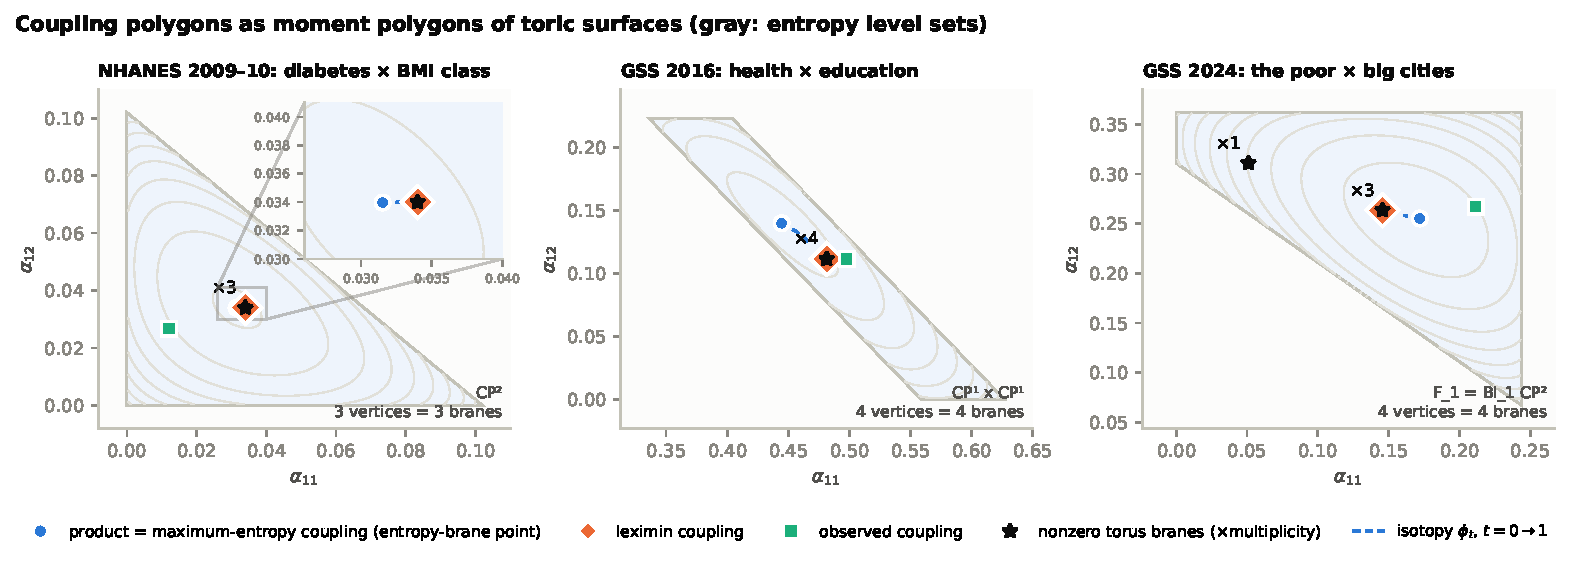
\includegraphics[width=\linewidth]{figs/fig_toric.pdf}
\caption{Coupling polygons of real $2\times3$ margins as moment polygons, with the nonzero torus branes of \cref{thm:sweep23}, the product
and leximin couplings, the observed coupling and the isotopy of \cref{prop:sheaf} \cite{Validation}.}\label{fig:publictoric}
\end{figure}

\begin{figure}[ht]
\centering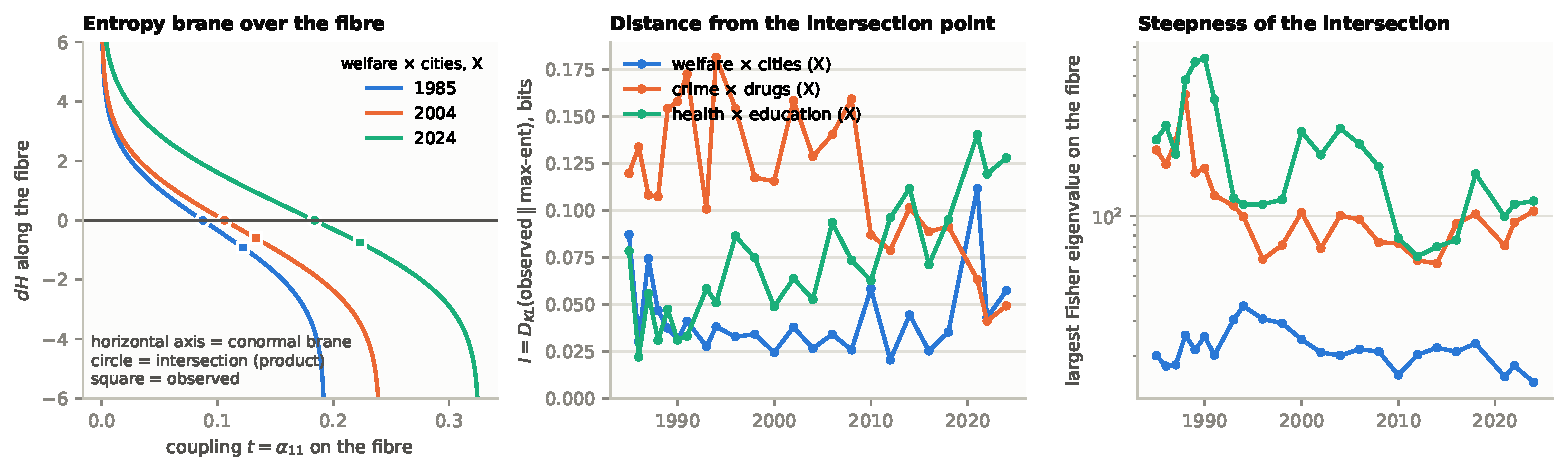
\includegraphics[width=\linewidth]{figs/fig_entropy_brane.pdf}
\caption{The entropy brane on survey margins: its intersection with the conormal brane (left), the divergence of the observed coupling from
the intersection point (middle), and the steepness of the intersection (right) \cite{Validation}.}\label{fig:publicbrane}
\end{figure}

\subsection{What the layers prove}

For $2\times3$ couplings the Fano layer gives the number of nonzero torus branes for all rational margins and their kinds for generic ones,
rules out the product coupling when its smallest facet cell is unique, and locates the branes exactly in
every computed case, where the leximin coupling always carries one (\cref{thm:sweep23}). Layer V removes the expected obstacle for every $3\times3$ margin: the
potential has no corrections (\cref{thm:nocorr}), so the same computation applies there, and \cref{ex:hf33crit} carries it out for one
example. Layer VI gives the topology and the monotone cases of the real locus, and isolates what is open, the Maslov-$1$ and Maslov-$0$ discs.
Layer VII reduces the sheaf model of the entropy brane to the admissibility of one explicit isotopy. The circulation obstruction of
\cref{thm:integral} is a separate statement about gluing, and none of the wall-crossings above is identified with it, or with the horn
obstructions of \cite[Prop.~6.2]{Bands}.

%=====================================================================
\section{Open problems}\label{sec:open}
%=====================================================================

\begin{enumerate}[leftmargin=*]
\item \emph{Real and torus branes.} Compute $HF(X^{\R}_{f,g},L_u)$ beyond the $2\times2$ case of \cref{prop:hf22}, over $\Z/2$ as in
  \cite{AlstonAmorim2012}, starting with the $2\times3$ branes of \cref{thm:sweep23} and with \cref{ex:hf33},
  with its products, and decide whether some refinement, for example a filtration by the sign pattern of the $2^d$ generators, sees
  positivity.
\item \emph{Contextuality with uncertain direct influences.} Build the posterior over the direct influences and the contextuality
  jointly (\cref{sec:cbd}), with a prior on consistent connectedness, and derive the sample size at which the decision of \cref{sec:cbd}
  stabilizes; relate the CbD degree to the contextual fraction beyond cyclic systems.
\item \emph{Non-equivariant correspondences.} \Cref{thm:integral} rules out equivariant ones. Is there a Lagrangian correspondence, not
  torus-equivariant, whose composition matches gluing with a stochastic kernel?
\item \emph{Bulk deformations.} For the $\mathrm{Bl}_2\mathbb{CP}^2$ and $\mathrm{Bl}_3\mathbb{CP}^2$ chambers of \cref{thm:sweep23}, find the
  bulk-balanced fibres of \cite{FOOO2011} and decide whether they form a continuum for Kähler structures that come from margins; and decide whether
  some bulk class makes the product coupling's brane nonzero.
\item \emph{Larger tables.} Prove \cref{thm:sweep23}(ii)--(iv) for all $2\times3$ margins rather than one representative per chamber, carry the sweep
  through the chambers of $3\times3$ margins, where by \cref{thm:nocorr} no corrections are needed, and decide whether the leximin coupling always
  carries at least half of the nonzero branes \cite[Obs.~10.10]{Conditionals}.
\item \emph{The real locus.} Compute the Floer cohomology of $X^{\R}_{f,g}$ over $\Z/2$ in the $\mathbb F_1$, $\mathrm{Bl}_2$ and $\mathrm{Bl}_3$ chambers,
  where it bounds Maslov-$1$ discs, and for $3\times3$, where it bounds Maslov-$0$ discs (\cref{prop:reallocus}).
\item \emph{The sheaf model.} Decide whether the isotopy of \cref{prop:sheaf} is admissible in the sense of \cite{NadlerZaslow2009}, so that the
  entropy brane can be replaced by the standard object of the open simplex.
\item \emph{The three-bit brane under noise.} Track the conormal brane of \cref{ex:threebits} as a family over $\varepsilon$, through the
  threshold, as a first example of a brane that disappears at a breaking point.
\end{enumerate}

%=====================================================================
\section{Computational checks}\label{sec:code}
%=====================================================================

All code is at \url{https://github.com/vkawasth/Trainingless-Transformer-NoGradientDescent/tree/main/bridges}, with the scripts of \cref{sec:modular} in its folder \texttt{fukaya}. \texttt{check\_bridges.py} runs sixteen checks, all passing: G1 (\cref{prop:fisher}); G2 (\cref{thm:conormal,cor:filler}); W1
(\cref{ex:threebits}, all five parts); S1 (the synthetic detection test, with joint and with pairwise-only samples); G3 (\cref{thm:abreu}, the determinant condition at every vertex
of an example with non-facet cells); W2 (\cref{ex:twobytwo}); G4 (\cref{thm:integral}); W3 (\cref{ex:gluetwo}); W4 (\cref{prop:morita}, the
dimension and the centre); H1 (\cref{ex:hf33}); H2 (\cref{prop:hf22}(ii), the displacement criterion); K1 (\cref{sec:cbd}: the linear program against the cyclic criterion, \cref{ex:cbd3},
and the posterior table, from \texttt{cbd/cbd.py}); F1 (\cref{prop:fano23,thm:sweep23,prop:reallocus}(i): the exact counts at $T=1$ for all $18$ facet sets, by \texttt{fukaya/t1\_exact.py};
the exact positions of the $18$ representatives recomputed and compared with the saved sweep of \texttt{fukaya/sweep23.py}, which takes about twelve
minutes; and the saved random study of \texttt{fukaya/random23.py}); F2 (\cref{prop:semifano33,thm:nocorr,prop:reallocus}(ii), in all $342$ chambers, by
\texttt{fukaya/all33.py}, \texttt{fukaya/nef33.py} and \texttt{fukaya/clt33.py}); F3 (\cref{ex:hf33crit}: the Krawczyk certificate of
\texttt{fukaya/krawczyk33.py}, the exact leading-order counts, and the saved continuation of \texttt{fukaya/deep33.py}); F4 (\cref{prop:sheaf}(i), by \texttt{fukaya/sheaf\_isotopy.py}).

\begin{thebibliography}{99}

\bibitem{Algebras}
V.~K. Awasthi, Coupling algebras: gluing, the square-zero cone and the ring of contingency tables. Technical report, Johns
Hopkins University, October 2026. Draft 4. Code: \url{https://github.com/vkawasth/Trainingless-Transformer-NoGradientDescent/tree/main/coupling_algebra}.

\bibitem{Bands}
V.~K. Awasthi, Bands: perturbation, tearing and breaking of coupling structures, and the entropy of changing probabilities.
Technical report, Johns Hopkins University, October 2026. Draft 2. Code: \url{https://github.com/vkawasth/Trainingless-Transformer-NoGradientDescent/tree/main/bands}.

\bibitem{Conditionals}
V.~K. Awasthi, Conditionals, couplings and toric geometry: kernels, the coupling nerve, cumulants and a {F}ukaya
programme. Technical report, Johns Hopkins University, October 2026. Revised draft 4. Code: \url{https://github.com/vkawasth/Trainingless-Transformer-NoGradientDescent/tree/main/conditionals}.

\bibitem{AbramskyBarbosaMansfield2017}
S.~Abramsky, R.~S. Barbosa and S.~Mansfield, Contextual fraction as a measure of contextuality. \emph{Phys. Rev. Lett.}
\textbf{119} (2017), 050504.

\bibitem{Abreu2003}
M.~Abreu, Kähler geometry of toric manifolds in symplectic coordinates. In \emph{Symplectic and Contact Topology}, Fields Inst.
Commun. 35, Amer. Math. Soc., 2003, 1--24.

\bibitem{ChoOh2006}
C.-H. Cho and Y.-G. Oh, Floer cohomology and disc instantons of Lagrangian torus fibers in Fano toric manifolds. \emph{Asian J.
Math.} \textbf{10} (2006), 773--814.

\bibitem{Csiszar1975}
I.~Csiszár, {$I$}-divergence geometry of probability distributions and minimization problems. \emph{Ann. Probab.} \textbf{3}
(1975), 146--158.

\bibitem{AbramskyBrandenburger2011}
S.~Abramsky and A.~Brandenburger, The sheaf-theoretic structure of non-locality and contextuality. \emph{New J. Phys.} \textbf{13}
(2011), 113036.

\bibitem{Delzant1988}
T.~Delzant, Hamiltoniens périodiques et images convexes de l'application moment. \emph{Bull. Soc. Math. France} \textbf{116}
(1988), 315--339.

\bibitem{DzhafarovKujala2016}
E.~N. Dzhafarov and J.~V. Kujala, Context-content systems of random variables: the Contextuality-by-Default theory. \emph{J. Math.
Psych.} \textbf{74} (2016), 11--33.

\bibitem{FOOO2010}
K.~Fukaya, Y.-G. Oh, H.~Ohta and K.~Ono, Lagrangian Floer theory on compact toric manifolds {I}. \emph{Duke Math. J.} \textbf{151}
(2010), 23--174.

\bibitem{Family}
V.~K. Awasthi, Coupling polytopes and toric geometry: the $2\times3$ family, the square case, higher levels and stability.
Companion paper, Johns Hopkins University, October 2026. Code: \url{https://github.com/vkawasth/Trainingless-Transformer-NoGradientDescent/tree/main/coupling}.

\bibitem{Fulton1993}
W.~Fulton, \emph{Introduction to Toric Varieties}, Annals of Mathematics Studies 131, Princeton University Press, 1993.

\bibitem{Guillemin1994}
V.~Guillemin, Kaehler structures on toric varieties. \emph{J. Differential Geom.} \textbf{40} (1994), 285--309.

\bibitem{ThreeLayers}
V.~K. Awasthi, Three layers of realisation: hierarchy recovery, holonomy, information, contextuality and categorical
dynamics. Technical report, Johns Hopkins University, revised October 2026. DOI: 10.13140/RG.2.2.24274.52163. Code: \url{https://github.com/vkawasth/Trainingless-Transformer-NoGradientDescent/tree/main/AMB-Vigneaux/}.

\bibitem{Keller2006}
B.~Keller, On differential graded categories. In \emph{Proceedings of the International Congress of Mathematicians, Madrid 2006},
Vol.~II, European Mathematical Society, 2006, 151--190.

\bibitem{KujalaDzhafarov2016}
J.~V. Kujala and E.~N. Dzhafarov, Proof of a conjecture on contextuality in cyclic systems with binary variables. \emph{Found. Phys.}
\textbf{46} (2016), 282--299.

\bibitem{KujalaDzhafarov2019}
J.~V. Kujala and E.~N. Dzhafarov, Measures of contextuality and non-contextuality. \emph{Philos. Trans. R. Soc. A} \textbf{377} (2019),
20190149.

\bibitem{Kushnirenko1976}
A.~G. Kushnirenko, Newton polytopes and the Bezout theorem. \emph{Funct. Anal. Appl.} \textbf{10} (1976), 233--235.

\bibitem{McDuffSalamon2017}
D.~McDuff and D.~Salamon, \emph{Introduction to Symplectic Topology}, 3rd ed., Oxford University Press, 2017.

\bibitem{AFOOO2026}
M.~Abouzaid, K.~Fukaya, Y.-G. Oh, H.~Ohta and K.~Ono, Quantum cohomology and split generation in Lagrangian Floer theory.
Preprint, arXiv:2606.12257, 2026.

\bibitem{Alston2010}
G.~Alston, Floer cohomology of real Lagrangians in the Fermat quintic threefold. Preprint, arXiv:1010.4073.

\bibitem{AlstonAmorim2012}
G.~Alston and L.~Amorim, Floer cohomology of torus fibers and real Lagrangians in Fano toric manifolds. \emph{Int. Math. Res. Not.
IMRN} \textbf{2012}, no.~12, 2751--2793.

\bibitem{Batyrev1993}
V.~V. Batyrev, Quantum cohomology rings of toric manifolds. \emph{Astérisque} \textbf{218} (1993), 9--34.

\bibitem{CLLT2017}
K.~Chan, S.-C. Lau, N.~C. Leung and H.-H. Tseng, Open Gromov--Witten invariants, mirror maps, and Seidel representations for toric
manifolds. \emph{Duke Math. J.} \textbf{166} (2017), 1405--1462.

\bibitem{Bernstein1975}
D.~N. Bernstein, The number of roots of a system of equations. \emph{Funct. Anal. Appl.} \textbf{9} (1975), 183--185.

\bibitem{Cho2005}
C.-H. Cho, Products of Floer cohomology of torus fibers in toric Fano manifolds. \emph{Comm. Math. Phys.} \textbf{260} (2005),
613--640.

\bibitem{CoxLittleSchenck2011}
D.~A. Cox, J.~B. Little and H.~K. Schenck, \emph{Toric Varieties}. Grad. Stud. Math. 124, Amer. Math. Soc., 2011.

\bibitem{DavisJanuszkiewicz1991}
M.~W. Davis and T.~Januszkiewicz, Convex polytopes, Coxeter orbifolds and torus actions. \emph{Duke Math. J.} \textbf{62} (1991),
417--451.

\bibitem{EvansLekili2019}
J.~D. Evans and Y.~Lekili, Generating the Fukaya categories of Hamiltonian $G$-manifolds. \emph{J. Amer. Math. Soc.} \textbf{32}
(2019), 119--162.

\bibitem{Floer1989}
A.~Floer, Witten's complex and infinite-dimensional Morse theory. \emph{J. Differential Geom.} \textbf{30} (1989), 207--221.

\bibitem{FOOO2011}
K.~Fukaya, Y.-G. Oh, H.~Ohta and K.~Ono, Lagrangian Floer theory on compact toric manifolds {II}: bulk deformations.
\emph{Selecta Math. (N.S.)} \textbf{17} (2011), 609--711.

\bibitem{FOOO2016}
K.~Fukaya, Y.-G. Oh, H.~Ohta and K.~Ono, Lagrangian Floer theory and mirror symmetry on compact toric manifolds. \emph{Astérisque}
\textbf{376} (2016).

\bibitem{FOOO2017}
K.~Fukaya, Y.-G. Oh, H.~Ohta and K.~Ono, Anti-symplectic involution and Floer cohomology. \emph{Geom. Topol.} \textbf{21} (2017),
1--106.

\bibitem{Haug2013}
L.~Haug, On the quantum homology of real Lagrangians in Fano toric manifolds. \emph{Int. Math. Res. Not. IMRN} \textbf{2013}, no.~14,
3171--3220.

\bibitem{McDuff2011}
D.~McDuff, Displacing Lagrangian toric fibers via probes. In \emph{Low-dimensional and Symplectic Topology}, Proc. Sympos. Pure Math.
82, Amer. Math. Soc., 2011, 131--160.

\bibitem{Nadler2009}
D.~Nadler, Microlocal branes are constructible sheaves. \emph{Selecta Math. (N.S.)} \textbf{15} (2009), 563--619.

\bibitem{NadlerZaslow2009}
D.~Nadler and E.~Zaslow, Constructible sheaves and the Fukaya category. \emph{J. Amer. Math. Soc.} \textbf{22} (2009), 233--286.

\bibitem{NakayamaNishimura2005}
H.~Nakayama and Y.~Nishimura, The orientability of small covers and coloring simple polytopes. \emph{Osaka J. Math.} \textbf{42}
(2005), 243--256.

\bibitem{Oh1993}
Y.-G. Oh, Floer cohomology of Lagrangian intersections and pseudo-holomorphic disks {II}: $(\mathbb{CP}^n,\mathbb{RP}^n)$.
\emph{Comm. Pure Appl. Math.} \textbf{46} (1993), 995--1012.

\bibitem{Pozniak1999}
M.~Po\'zniak, Floer homology, Novikov rings and clean intersections. In \emph{Northern California Symplectic Geometry Seminar},
Amer. Math. Soc. Transl. Ser.~2, 196, 1999, 119--181.

\bibitem{Ritter2016}
A.~F. Ritter, Circle-actions, quantum cohomology, and the Fukaya category of Fano toric varieties. \emph{Geom. Topol.} \textbf{20}
(2016), 1941--2052.

\bibitem{Walcher2007}
J.~Walcher, Opening mirror symmetry on the quintic. \emph{Comm. Math. Phys.} \textbf{276} (2007), 671--689.

\bibitem{Validation}
V.~K. Awasthi, Empirical site separation: bending, tearing, contextuality and holonomy in a national survey, retrained language models and
clinical data. Technical report, Johns Hopkins University, October 2026. Code: \url{https://github.com/vkawasth/Trainingless-Transformer-NoGradientDescent/tree/main/monitor}.

\end{thebibliography}
\end{document}
